\documentclass{article}

\usepackage[margin=1.75cm]{geometry}
\usepackage{graphicx}
\usepackage{pgfplots}
\usepackage{epstopdf}
\usepackage{xcolor}
\usepackage{tikz}
\usepackage{amsmath}

\usepackage{subcaption}
\usepackage{hyperref}
\usepackage{multirow}
\usepackage{inputenc}
\usepackage{babel}

\usetikzlibrary{arrows.meta, patterns}

\pgfplotsset{compat=1.18}

\title{H1 – Testing standard benchmark functions \\ Hill-Climbing and Simulated annealing}
\author{Dinca Georgian(2E2) - Brahă Petru(2E3)}
\date{October 27, 2024}

%%------------------------------------------------
%% actual document:

\begin{document}

\maketitle

\section{Abstract}

This research document contains a comparative analysis of local search strategies applied to four optimization benchmark functions: \textbf{Sphere}, \textbf{Rastrigin}, \textbf{Schwefel} and \textbf{Michalewicz}. Three search strategies are evaluated - \textit{\textbf{First Improvement}}, \textit{\textbf{Best Improvement}}, and \textit{\textbf{Simulated Annealing}}, across the following problem dimensions (\textbf{10D}, \textbf{30D}, and \textbf{100D}), with an additional investigation of \textit{\textbf{Worst Improvement}} strategy for the lower-dimensional cases (\textbf{10D} and \textbf{30D}). In addition to solution quality, the execution times of each strategy were recorded and compared. Results and findings from these experiments are presented and discussed.


\section{Introduction}

The desired goal for our program is to find the minimum point for the four matemathical functions. Why is it difficult?\\
As we have seen from the previous paper (H0), achieving perfect results or using a deterministic approach is time-consuming and not fesable. These functions pose challenges due to their complex landscapes and multiple local optima. To address this challenge, we employ two popular optimization algorithms: Hill Climbing and Simulated Annealing. The Hill Climbing algorithm explores different improvement strategies, while Simulated Annealing utilizes a probabilistic approach, its role is to hybridized.

%%------------------------------------------------
%% explanations:

\section{Method}

For each of the function we analyses each of the four approaches. for each of them a sample of 30 outputs is computed. One value out of sample is resulted after 10.000 iterations of the algorithm Hill Climbing. 

Where we have chosen the precision as -5 throughout of the entire experimentation.\\
We will not go into details with the algorithm with bitstrings, neighborhood, etc. 
There should be 30 global outputs and the result of the algorithm is the best soltuion out of those. \\ 

Simulated Annealing uses the same principles as Hill Climber but is more precise in most cases because it utilizes the concept of temperature. Evading from local minimum to a potential better value.
Again we will not go into details about the principles and the implementation behind.

\subsection{Setup}
The algorithms have been implemented to leverage GPU acceleration by using NVIDIA's CUDA framework. The system was equipped with an RTX 4090 graphics card, mobile version. The parallel nature of local search algorithms, where multiple independent search iterations can be executed simultaneously, makes them particularly well-suited for GPU implementation due to their architecture having very large number of cores and threads that can run in parallel. Each search iteration operates independently on its own thread, which parallelizes the workload efficiently. \\ \\
Our GPU implementation utilizes a thread organization scheme of 32 threads per block, aligning with the NVIDIA warp size for optimal execution efficiency. This configuration minimizes thread divergence and maximizes memory coalescing [https://docs.nvidia.com/cuda/cuda-c-best-practices-guide/index.html\# coalesced-access-to-global-memory], resulting in improved computational performance. Each experimental configuration executes 20,000 iterations per sample, with 30 independent samples for statistical robustness. Results are reported with 5 digits of precision.

\subsection{Simulated Annealing Implementation}
Our implementation features a hybrid approach that combines traditional SA with a Best Improvement local search phase after the temperature drops and it can no longer escape the local optimum. The initial temperature $T_0$ is dynamically calculated based on the dimension number using the formula $T_0 = \left|\frac{40n}{\ln(0.8)}\right|$, where n is the number of dimensions. This adaptive initial temperature ensures appropriate scaling of the acceptance probability across different problem dimensions. \\ \\
The cooling schedule is implemented with a geometric decay and a cooling rate of 0.985, maintaining a balance between exploration and exploitation. The algorithm progresses until either the temperature falls below a threshold of $T_0\times10^{-8}$, or when the search stagnates for 4 consecutive temperature changes. For each temperature, we attempt to achieve 20n successful moves, where n is the number of dimensions, with a maximum of 200n total attempts per temperature to prevent excessive computation in flat regions of the search space. \\ \\
The solution representation uses a binary encoding, with neighborhood moves implemented as single bit-flips. Move acceptance follows the standard Metropolis criterion:
\begin{itemize}
    \item Improvements are always accepted
    \item Deteriorating moves are accepted with probability $\exp\left(-\frac{| \Delta f |}{T}\right)$, where $\Delta f$ is the absolute fitness difference and T is the current temperature
\end{itemize}


\section{Experiment}

To evaluate the performance of the Hill Climbing and Simulated Annealing algorithms in finding the minimum values for the De Jong 1, Schwefel’s, Rastrigin’s, and Michalewicz’s functions, I’ve conducted a series of experiments. The experiments were conducted on functions with dimensions of 5, 10, and 30. The precision of at least 5 decimal places after 0 was maintained throughout the experimentation. \\

For each function and dimension, the program executed the following steps:
1. Initialization.
a) Randomly generated an initial solution within the search space boundaries.
2. Hill Climbing.
a) Applied the best improvement variant of the Hill Climbing algorithm.
b) Iteratively selected a neighboring solution and evaluated it.
c) If the evaluation of the neighboring solution was better, it was accepted as the new current solution.
d) The process continued until no better solution was found, or a termination condition was met.
e) Repeated the Hill Climbing process with the first improvement and
worst improvement variants.
3. Simulated Annealing.
a) Hybridized the Simulated Annealing algorithm with the best improvement variant of Hill Climbing.
b) Defined an initial temperature and cooling schedule.
c) Iteratively generated a neighboring solution and evaluated it.
d) Compared the evaluation of the neighboring solution with the current solution.
e) Accepted the neighboring solution if it was better or based on a probability criterion influenced by the temperature and the difference in evaluation between the solutions.
f) Adjusted the temperature according to the cooling schedule until a termination condition was met.
4. Performance Evaluation.
a) Recorded the best evaluated value obtained by each algorithm for each function and dimension.
b) Repeated the experiments multiple times to record all the results.
This experiment was implemented using C++ programming language.

%%------------------------------------------------
%% end of raport:

\newpage
\section{Results}

%%------------------------------------------------

\subsection{Sphere}
%$$f(\mathbf{x}) = \sum_{i=1}^{n} x_i^2 , x_i \in \left[ -5.12, 5.12 \right] $$

%%------------------------------------------------

\begin{figure}[!h]
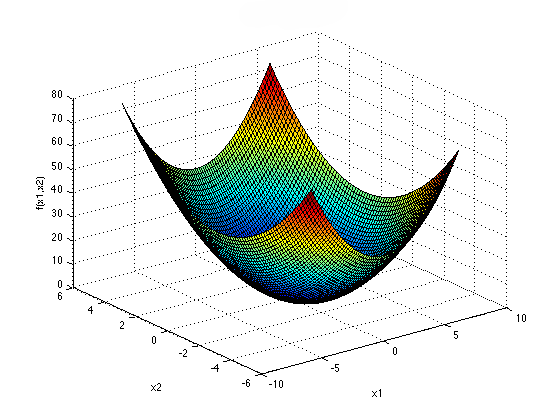
\includegraphics[width=\textwidth,height=\textheight,keepaspectratio]{sphere.png}
  \caption{Sphere's 2-dimensional graph function \cite{sf-uni-sp}}
\end{figure}

%%------------------------------------------------
 
\begin{table}[htbp]
\begin{minipage}{.4\linewidth}
    \centering

    \begin{tabular}{|c|c|c|c|c|}
    \hline
    D   & $\sigma$  & avg. time     & avg. sol.     & best sol. \\
    \hline
    10  & 0         & 0             & 0             & 0 \\
    \hline
    30  & 0         & 0             & 0             & 0 \\
    \hline
    100 & 0         & 0             & 0             & 0 \\
    \hline
    \end{tabular}
    \caption{Best improvement}
  \end{minipage}%
  \quad % ----------------------------------
  \begin{minipage}{.75\linewidth}
    \centering

    \begin{tabular}{|c|c|c|c|c|}
    \hline
    D   & $\sigma$  & avg. time     & avg. sol.     & best sol. \\
    \hline
    10  & 0         & 0             & 0             & 0 \\
    \hline
    30  & 0         & 0             & 0             & 0 \\
    \hline
    100 & 0         & 0             & 0             & 0 \\
    \hline
    \end{tabular}
    \caption{First improvement}
  \end{minipage}
\end{table}
\begin{table}[!htbp]
\begin{minipage}{.4\linewidth}
    \centering

    \begin{tabular}{|c|c|c|c|c|}
    \hline
    D   & $\sigma$  & avg. time     & avg. sol.     & best sol. \\
    \hline
    10  & 0         & 0             & 0             & 0 \\
    \hline
    30  & 0         & 0             & 0             & 0 \\
    \hline
    \end{tabular}
    \caption{Worst improvement}
  \end{minipage}%
  \quad % ----------------------------------
  \begin{minipage}{.75\linewidth}
    \centering

    \begin{tabular}{|c|c|c|c|c|}
    \hline
    D   & $\sigma$  & avg. time     & avg. sol.     & best sol. \\
    \hline
    10  & 0         & 0             & 0             & 0 \\
    \hline
    30  & 0         & 0             & 0             & 0 \\
    \hline
    100 & 0         & 0             & 0             & 0 \\
    \hline
    \end{tabular}
    \caption{Simulated annealing}
  \end{minipage}
\end{table}

\newpage
\setcounter{table}{0}

%%------------------------------------------------

\subsection{Rastrigin}
$$ f(x) = A \cdot n + \sum_{i=1}^n \left[ x_i^2 - 10 \cdot cos(2 \pi x_i) \right] , x_i \in \left[ -5.12, 5.12 \right] $$

%%------------------------------------------------

\begin{figure}[!h]
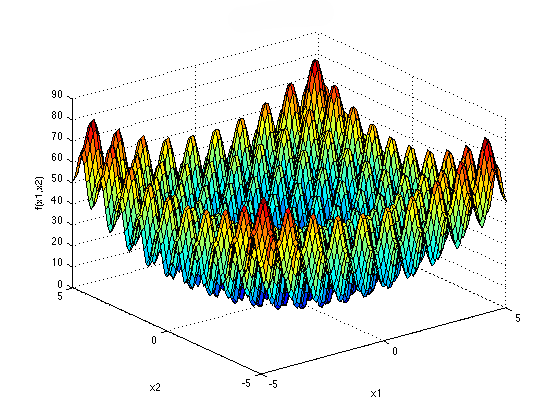
\includegraphics[width=\textwidth,height=\textheight,keepaspectratio]{rastrigin.png}
  \caption{Rastrigin's 2-dimensional graph function \cite{sf-uni-ra}}
\end{figure}

%%------------------------------------------------

\begin{table}[htbp]
\begin{minipage}{.4\linewidth}
    \centering
    
    \begin{tabular}{|c|c|c|c|c|}
    \hline
    D   & $\sigma$  & avg. time     & avg. sol.     & best sol.\\
    \hline
    10  & 0         & 307.48056ms   & 1.96332       & 0.99496 \\
    \hline
    30  & 0         & 7749.7280ms   & 22.49692      & 16.15900 \\
    \hline
    100 & 0         & 271917.65625ms& 124.04872     & 103.27991 \\
    \hline
    \end{tabular}
    \caption{Best improvement}
  \end{minipage}%
  \quad % ----------------------------------
  \begin{minipage}{.75\linewidth}
    \centering
    
    \begin{tabular}{|c|c|c|c|c|}
    \hline
    D   & $\sigma$  & avg. time     & avg. sol.     & best sol. \\
    \hline
    10  & 0         & 182.90204ms   & 3.42327       & 1.23582 \\
    \hline
    30  & 0         & 4375.91602ms  & 29.97694      & 22.84631 \\
    \hline
    100 & 0         & 154125.26562ms& 155.08213     & 141.60620 \\
    \hline
    \end{tabular}
    \caption{First improvement}
  \end{minipage}
\end{table}
\begin{table}[!htbp]
\begin{minipage}{.4\linewidth}
    \centering

    \begin{tabular}{|c|c|c|c|c|}
    \hline
    D   & $\sigma$  & avg. time     & avg. sol.     & best sol. \\
    \hline
    10  & 0         & 2519.98950ms  & 5.12165       & 3.00004 \\
    \hline
    30  & 0         & 57137.27734ms & 38.18328      & 29.23457 \\
    \hline
    \end{tabular}
    \caption{Worst improvement}
  \end{minipage}%
  \quad % ----------------------------------
  \begin{minipage}{.75\linewidth}
    \centering

    \begin{tabular}{|c|c|c|c|c|}
    \hline
    D   & $\sigma$  & avg. time     & avg. sol.     & best sol. \\
    \hline
    10  & 0         & 19811.83398ms & 0.00000       & 0.00000 \\
    \hline
    30  & 0         & 171314ms      & 6.20453       & 3.99499 \\
    \hline
    100 & 0         & 1150011.1250ms& 47.64466      & 40.26256 \\
    \hline
    \end{tabular}
    \caption{Simulated annealing}
  \end{minipage}
\end{table}

\newpage
\setcounter{table}{0}

%%------------------------------------------------

\subsection{Schwefel}
$$f(\mathbf{x}) = -\sum_{i=1}^{n} x_i \cdot \sin\left(\sqrt{|x_i|}\right) , x_i \in \left[-500,500\right]$$

%%------------------------------------------------

\begin{figure}[!h]
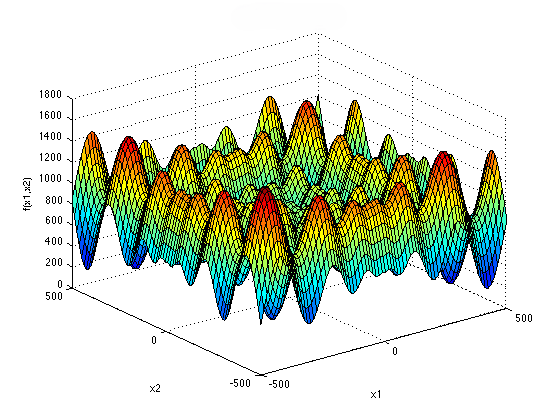
\includegraphics[width=\textwidth,height=\textheight,keepaspectratio]{schwefel.png}
  \caption{Schwefel's 2-dimensional graph function \cite{sf-uni-sw}}
\end{figure}
\vspace{0.5cm}

%%------------------------------------------------

\begin{table}[htbp]
\begin{minipage}{.4\linewidth}
    \centering

    \begin{tabular}{|c|c|c|c|c|}
    \hline
    D   & $\sigma$  & avg. time     & avg. sol.     & best sol. \\
    \hline
    10  & 0         & 0             & 0             & 0 \\
    \hline
    30  & 0         & 0             & 0             & 0 \\
    \hline
    100 & 0         & 0             & 0             & 0 \\
    \hline
    \end{tabular}
    \caption{Best improvement}
  \end{minipage}%
  \quad % ----------------------------------
  \begin{minipage}{.75\linewidth}
    \centering

    \begin{tabular}{|c|c|c|c|c|}
    \hline
    D   & $\sigma$  & avg. time     & avg. sol.     & best sol. \\
    \hline
    10  & 0         & 0             & 0             & 0 \\
    \hline
    30  & 0         & 0             & 0             & 0 \\
    \hline
    100 & 0         & 0             & 0             & 0 \\
    \hline
    \end{tabular}
    \caption{First improvement}
  \end{minipage}
\end{table}
\begin{table}[!htbp]
\begin{minipage}{.4\linewidth}
    \centering

    \begin{tabular}{|c|c|c|c|c|}
    \hline
    D   & $\sigma$  & avg. time     & avg. sol.     & best sol. \\
    \hline
    10  & 0         & 0             & 0             & 0 \\
    \hline
    30  & 0         & 0             & 0             & 0 \\
    \hline
    100 & 0         & 0             & 0             & 0 \\
    \hline
    \end{tabular}
    \caption{Worst improvement}
  \end{minipage}%
  \quad % ----------------------------------
  \begin{minipage}{.75\linewidth}
    \centering

    \begin{tabular}{|c|c|c|c|c|}
    \hline
    D   & $\sigma$  & avg. time     & avg. sol.     & best sol. \\
    \hline
    10  & 0         & 0             & 0             & 0 \\
    \hline
    30  & 0         & 0             & 0             & 0 \\
    \hline
    100 & 0         & 0             & 0             & 0 \\
    \hline
    \end{tabular}
    \caption{Simulated annealing}
  \end{minipage}
\end{table}

\newpage
\setcounter{table}{0}

%%------------------------------------------------

\subsection{Michalewicz}
$$f(\mathbf{x}) = -\sum_{i=1}^{n} \sin(x_i) \cdot \left(\sin\left(ix_i^2 / \pi\right)\right)^{2m} , m = 10, x_i \in \left[0,\pi\right]$$

%%------------------------------------------------

\begin{figure}[!h]
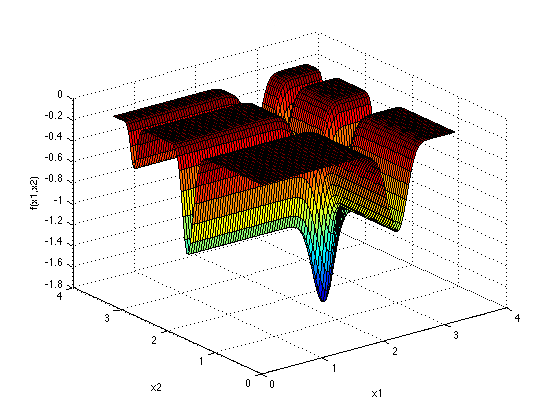
\includegraphics[width=\textwidth,height=\textheight,keepaspectratio]{michalewicz.png}
  \caption{Michalewicz's 2-dimensional graph function \cite{sf-uni-mc}}
\end{figure}
\vspace{0.5cm}

%%------------------------------------------------

\begin{table}[htbp]
\begin{minipage}{.4\linewidth}
    \centering

    \begin{tabular}{|c|c|c|c|c|}
    \hline
    D   & $\sigma$  & avg. time     & avg. sol.     & best sol. \\
    \hline
    10  & 0         & 0             & 0             & 0 \\
    \hline
    30  & 0         & 0             & 0             & 0 \\
    \hline
    100 & 0         & 0             & 0             & 0 \\
    \hline
    \end{tabular}
    \caption{Best improvement}
  \end{minipage}%
  \quad % ----------------------------------
  \begin{minipage}{.75\linewidth}
    \centering

    \begin{tabular}{|c|c|c|c|c|}
    \hline
    D   & $\sigma$  & avg. time     & avg. sol.     & best sol. \\
    \hline
    10  & 0         & 0             & 0             & 0 \\
    \hline
    30  & 0         & 0             & 0             & 0 \\
    \hline
    100 & 0         & 0             & 0             & 0 \\
    \hline
    \end{tabular}
    \caption{First improvement}
  \end{minipage}
\end{table}
\begin{table}[!htbp]
\begin{minipage}{.4\linewidth}
    \centering

    \begin{tabular}{|c|c|c|c|c|}
    \hline
    D   & $\sigma$  & avg. time     & avg. sol.     & best sol. \\
    \hline
    10  & 0         & 0             & 0             & 0 \\
    \hline
    30  & 0         & 0             & 0             & 0 \\
    \hline
    100 & 0         & 0             & 0             & 0 \\
    \hline
    \end{tabular}
    \caption{Worst improvement}
  \end{minipage}%
  \quad % ----------------------------------
  \begin{minipage}{.75\linewidth}
    \centering

    \begin{tabular}{|c|c|c|c|c|}
    \hline
    D   & $\sigma$  & avg. time     & avg. sol.     & best sol. \\
    \hline
    10  & 0         & 0             & 0             & 0 \\
    \hline
    30  & 0         & 0             & 0             & 0 \\
    \hline
    100 & 0         & 0             & 0             & 0 \\
    \hline
    \end{tabular}
    \caption{Simulated annealing}
  \end{minipage}
\end{table}

%%------------------------------------------------

\subsection{Interpretation}

The experimental results demonstrate that \textit{\textbf{Best Improvement}} consistently outperforms \textit{\textbf{First Improvement}} in solution quality across all test functions, particularly in higher dimensions, however at a higher computational cost. \textit{\textbf{Simulated Annealing}} exhibits superior performance by escaping local optima, especially notable for \textbf{Rastrigin} and \textbf{Schwefel} functions, yielding better results when compared against \textit{\textbf{Best Improvement}}. Finally, \textit{\textbf{Worst Improvement}} showed inferior results at a higher computational cost than all other strategies.

\section{Conclusions}

After taking a look at the results we have obtained, we can safely say that the Hill Climber algorithm is a really efficient algorithm that manages to determine a solution that is really close to perfect answer in a reasonable amount of time. The exact time is way lower than iterating through the whole graph and comparable to that of a probabilistic algorithm.\\

We can also observe that Simulated Annealing provides us in a more restrained time interval with a usually better result, so it is definitely more useful in most cases to use this variant as opposed to Hill Climber (or a deterministic or heuristic approach).\\

The findings revealed that the choice of optimization algorithm and its variants significantly impacted the search for the global minimum. The Hill Climbing algorithm, with its first improvement, best improvement, and worst improvement variants, showcased different trade-offs between exploration and exploitation. Simulated Annealing, when hybridized with one of the Hill Climbing variants, demonstrated improved convergence properties. Overall, this research provides valuable insights into the application of optimization algorithms in solving complex optimization problems and contributes to the understanding of their performance across different dimensions.

%%------------------------------------------------
%% bibliography

\begin{thebibliography}{9}

\bibitem{sf-uni-sp}
  Simon Fraser University \\ Sphere's function.
  \url{https://www.sfu.ca/~ssurjano/spheref.html}

\bibitem{sf-uni-ra}
  Simon Fraser University \\  Rastrigin's function.
  \url{https://www.sfu.ca/~ssurjano/rastr.html}

\bibitem{sf-uni-sw}
  Simon Fraser University \\ Schwefel's function.
  \url{https://www.sfu.ca/~ssurjano/schwef.html}

\bibitem{sf-uni-mc}
  Simon Fraser University \\ Michalewicz's function.
  \url{https://www.sfu.ca/~ssurjano/michal.html}

\bibitem{}
  Croitoru Eugen - course \\ Hill Climbing documentation.
  \url{https://gitlab.com/eugennc/teaching/-/blob/master/GA/}

\bibitem{l}
  Overleaf \\ LaTeX training.
  \url{https://tex.stackexchange.com/questions/39017/how-to-influence-the-position-of-float-environments-like-figure-and-table-in-lat/39020#39020} \\
  \url{https://latex-cookbook.net/function-plot/} \\  \url{https://www.overleaf.com/learn/latex/Learn_LaTeX_in_30_minutes}

\end{thebibliography}  
\end{document}
